\documentclass[tikz,border=8pt]{standalone}
% Shared look for every TikZ diagram. Load with \input{../../tools/tikz-style.tex}
\usepackage[sfdefault]{roboto}
\usetikzlibrary{arrows.meta, positioning, shapes.geometric, calc, fit, backgrounds}
\definecolor{cblue}{HTML}{4C78A8}
\definecolor{corange}{HTML}{F58518}
\definecolor{cgreen}{HTML}{54A24B}
\definecolor{cred}{HTML}{E45756}
\definecolor{cpurple}{HTML}{B279A2}
\definecolor{cgrey}{HTML}{6B6B6B}
\tikzset{
  every picture/.style={font=\sffamily, line width=1.2pt},
  box/.style={draw=#1, fill=#1!12, rounded corners=4pt, align=center, inner sep=7pt, minimum height=1.1cm},
  box/.default=cgrey,
  arrow/.style={-{Stealth[length=3mm]}, draw=cgrey, line width=1.4pt},
  title/.style={font=\sffamily\bfseries\Large},
  note/.style={font=\sffamily\small, text=cgrey, align=center},
}
\AtBeginDocument{\hyphenpenalty=10000 \exhyphenpenalty=10000}

% Path coordinates of the car with its rear axle at (14.0, 0.0), heading 10 deg, on the course's arc (centre (10, 10),
% radius 10 m): nearest course point P = (13.714, 0.715) on the line from the centre through the car; distance along the
% course s = 10 + 10 x 0.3805 = 13.805 m; the course's heading at P 21.80 deg; tangent t and normal n at P (the Frenet
% frame; on an arc the normal points at the centre); lateral error e = 10 - 10.770 = -0.770 m (right of the course);
% heading error 10 - 21.80 = -11.80 deg.
\begin{document}
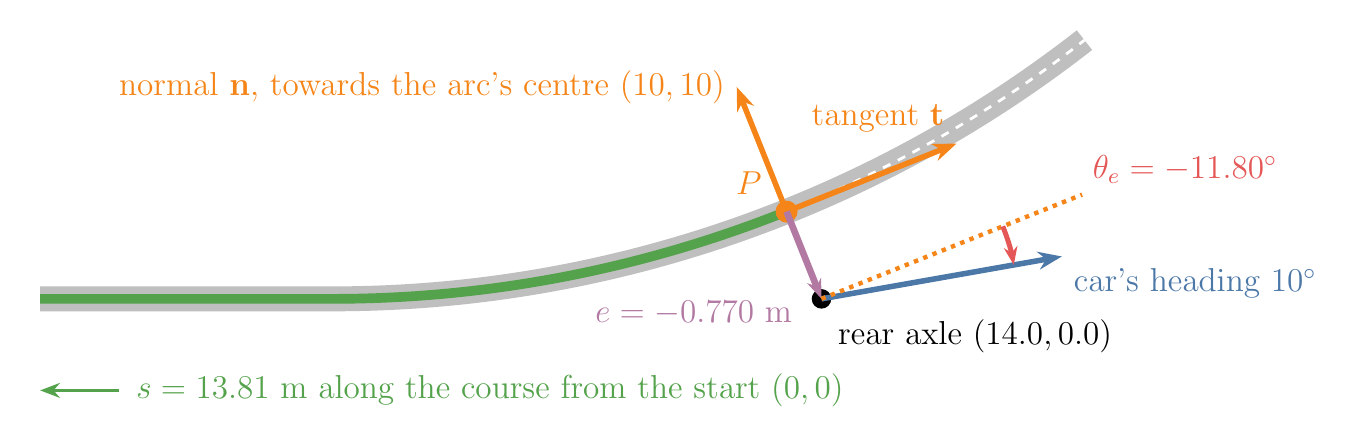
\begin{tikzpicture}[scale=1.55, every node/.append style={font=\large}]
  % the course: first straight (to x = 10) and the arc round (10, 10)
  \draw[black!25, line width=9pt] (7.6,0) -- (10,0) arc (-90:-52:10);
  \draw[white, dashed, line width=1pt] (7.6,0) -- (10,0) arc (-90:-52:10);
  % s so far: from the start, off the left edge, to P
  \draw[cgreen, line width=3.5pt] (7.6,0) -- (10,0) arc (-90:-68.1986:10);
  \draw[-{Stealth[length=2.5mm]}, cgreen, line width=1.2pt] (8.25,-0.75) -- (7.6,-0.75);
  \node[cgreen, anchor=west] at (8.3,-0.75) {$s = 13.81$ m along the course from the start $(0, 0)$};
  % Frenet frame at P: tangent (21.8 deg) and normal (111.8 deg)
  \coordinate (P) at (13.7139,0.7152);
  \draw[-{Stealth[length=3mm]}, corange, line width=2pt] (P) -- ++(21.8014:1.5) node[anchor=south east] {tangent $\mathbf t$};
  \draw[-{Stealth[length=3mm]}, corange, line width=2pt] (P) -- ++(111.8014:1.1) node[anchor=east] {normal $\mathbf n$, towards the arc's centre $(10, 10)$};
  \fill[corange] (P) circle (0.09);
  \node[corange, anchor=east] at (13.6,0.95) {$P$};
  % the car's rear axle and heading
  \coordinate (C) at (14,0);
  \fill[black] (C) circle (0.08);
  \draw[-{Stealth[length=3mm]}, cblue, line width=2pt] (C) -- ++(10:2.0) node[anchor=north west] {car's heading $10^\circ$};
  \node[anchor=north west] at (14.05,-0.08) {rear axle $(14.0, 0.0)$};
  % lateral error from P to the car
  \draw[-{Stealth[length=2.5mm]}, cpurple, line width=2.4pt] (P) -- (C);
  \node[cpurple, anchor=east] at (13.85,-0.12) {$e = -0.770$ m};
  % heading error: from the course's direction (dotted copy at the car) to the car's heading
  \draw[corange, dotted, line width=1.6pt] (C) -- ++(21.8014:2.3);
  \draw[-{Stealth[length=2.3mm]}, cred, line width=1.8pt] ($(C)+(21.8014:1.6)$) arc (21.8014:10:1.6);
  \node[cred, anchor=south west] at ($(C)+(21.8014:2.3)$) {$\theta_e = -11.80^\circ$};
\end{tikzpicture}
\end{document}
